\chapter{Introduction}

\section{Background to the Study}
Human motion capture systems are often very costly and confine the capture area to a certain confined space. These limitations prevent us from understanding bipedal motion in complex environments, knowledge that proves to be critical in the development of functional humanoid robotics. Examples of such systems can be seen in \cite{sandau2014markerless} where 8 cameras and stereo vision was used to recreate a 3D model of a walking person and in \cite{pfister2014comparative} where 10 Vicon cameras and a full body marked suit was used for the same objective.

A popular approach taken to overcome the spatial limitations inherent in camera based systems is the use of body mounted sensor networks. A commercial sensor suit developed by XSens and demonstrated in \cite{roetenberg2009xsens} can accurately recreate a 3D model of human motion using inertial sensors and data fusion. Similar work completed by Seel et al. \cite{seel2014imu} further proves the accuracy of such systems. Although the mentioned systems overcome the stated limitations; they do so at increased complexity and cost. They often lack modularity and their proprietary software is difficult to adapt.

\begin{figure}[!ht] 
\captionsetup{width=0.8\linewidth, font=small}  
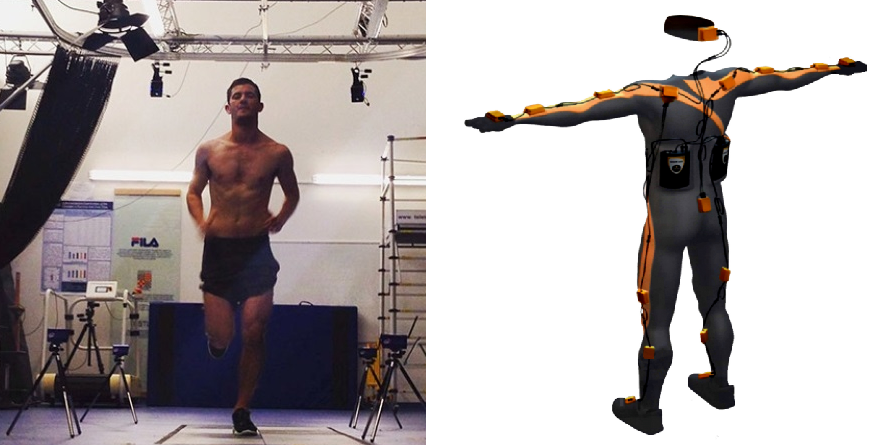
\includegraphics[width=0.5\linewidth]{figures/COMBO.png}
\caption{Left: Vicon motion capture system tracking the human gait (from \cite{roetenberg2009xsens}) Right: The Xsens MVN motion capture suit (from \cite{vicon})}
\label{fig:COMBO}
\end{figure}

Recent work \cite{patel2017trackingieee} completed by the Mechatronics Lab at the University of Cape Town showed data capture with both subject-borne cameras and sensors can be used to better understand unconstrained movement in a natural environment. This was based on research completed by Stocks \cite{bradstocks} at the same laboratory. The presented work showed the successful kinematic modelling of a cheetah (Acinonyx jubatus) tail whilst running freely. The importance of understanding motion in the natural world is outlined in \cite{patel2014rapid} and is the cornerstone of biomimicry as defined by \cite{benyus2002biomimicry}.

  
\section{Objectives of the Study}
Depth imagery in the field of human motion capture has been extensively reviewed in \cite{chen2013survey}, where the lack of data from complex movements in different environments is listed as a challenge. This reaffirms the difficulty stated in the previous section. Solely relying on motion sensors to understand the gait has been reviewed by \cite{picerno201725}. Although this approach was found to be accurate for external environments it has limitation with respect to cost and sensor disturbance. From these reviews it is clear that a middle ground must exist that can combine the strengths of both the approaches to provide a holistic solution.

This research project aims to show that subject-borne sensors, primarily a combination of cameras and IMUs, can provide researchers in the field of health sciences, biomechanics and biomimicry with extensive datasets to better understand and model the bipedal motion of humans. It builds on the foundational work presented by Stocks and Patel \cite{bradstocks} and envisions to implement a similar system to track data points on the lower limbs of a runner. The original prototype system is shown below, mounted to the back of a cheetah.

\begin{figure}[!ht] 
\captionsetup{width=0.8\linewidth, font=small}  
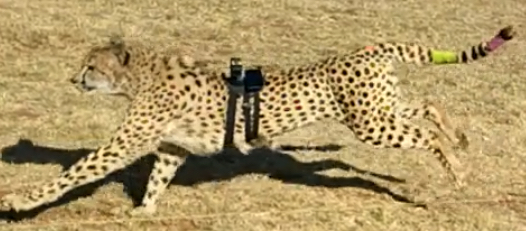
\includegraphics[width=0.9\linewidth]{figures/introcheetah.png}
\caption{A cheetah wearing the wearable motion capture system designed by Stocks \cite{bradstocks}}
\label{fig:introcheetah}
\end{figure}

This research project firstly aims to design such a data capture system using available hardware solutions and basic 3D printable components. By using such elements the system gains modularity whilst the overall cost and development time is reduced. This rapid prototyping philosophy was chosen such that the project could be completed within a 4 month time frame.

While developing and constructing the above mentioned system a basic model of the human lower limbs will be created. The model will need well defined mathematical definitions such that kinematic principles can be applied to quantify critical gait elements. Important simplifications and shortcomings of the model need to be explored and methods to minimize their effects created.

The design and software implementation of a system to extract, process and fuse the various data sources needs to be developed. This implementation will include, but is not limited to, an Extended Kalman filter and an image processing algorithm to identify critical points in the video data.

Finally this thesis will pay close attention to similarities in understanding the human gait using technologies used to control the dynamics of bipedal humanoid robots. Since these robots attempt to imitate human motion many of they key principles in the field of robotics relates directly to to the bio-mechanics of humans.

\section{Scope and Limitations}
The scope of this research is to model and estimate the human lower limbs during a flat ground steady state run. The motion will be estimated by determining the different joint angles as well as the motion of the runner w.r.t. the inertial frame. Joint angles are a popular method of quantization and the availability of rich datasets allow comparative analysis on the final findings of this work. This is the first logical step in the iterative design process to eventually understand movement in complex environments using wearable motion capture systems.

The availability of equipment also influenced the quality and accuracy of the system. Due to financial constraints the system was designed to use available hardware and minimize additional expenses. Although the the system designed cannot be classified as low cost, when compared to other methods of motion capture it becomes financially attractive. The components selected are also interchangeable and need not exactly match the specifications presented herein.

It should be noted that the research presented herein does not seek to push the boundaries of modern sensor technology, nor does it wish to re-imagine understood and accepted models of natural phenomena. Instead, a methodology is proposed that brings together elements from exciting disciplines of research such that richer datasets can be generated and studied. This research therefore serves as a proof of concept for a novel wearable motion capture technology.

There is another distinction to make with regard to scope of the project; that is the distinction between kinematics and dynamics. This project is aimed at understanding, modelling and estimating the kinematics of lower limbs, that is to say the movement and motion of the lower limbs but not the forces and torques causing them. These forces are important elements of motion, but require some adaptation to the proposed methodology to fully understand.

Furthermore this thesis will not compare different running styles or comment on their energy efficiency. Interpreting and rehabilitating the human gait is best left to medical professionals. This system may be applicable to work done in such professions, but the task of developing this system is one of engineering.

Finally a large portion of this project relies on software written for MathWorks' MATLAB \cite{matlab}. This software is single purpose and serves only this thesis. The software itself is not meant to be modular or generalized, yet can serve as a guideline for research using a similar methodology. The software can be found on the accompanying disc. Some software snippets of critical importance has been added to this thesis to highlight the important aspects of implementing the various mathematical constructs. The various Dassault Systèmes SOLIDWORKS \cite{solidworks} models are also present on the same disc. These models are also specific to this thesis and can only provide insight for adaptations. 

\section{Plan of Development}
The following chapter contains an extensive literature review where various methods of modelling and verifying the human gait has been discussed. There are also sections dedicated to subject borne data capture, computer vision, inertial measurement units (motion sensors), humanoid robotics and mathematical modelling.

This is followed by a chapter titled methodology that presents the the planning and ideation of the thesis. It serves as a link between the theoretical work presented in the literature review and the engineering approach and application detailed in the chapters that follow it. It lays out a plan and shows how engineering specifications were generated from a generally defined problem. 

The final three chapters that make up the body of this report are titled "Designing the Data Capture System", "Processing the Captured Data" and "Data Fusion and State Estimation" in order of appearance. True to their title they present the processes followed to complete the major milestones of the project.

In closing a chapter is dedicated to presenting and discussing the results obtained, followed by the final chapter that draws conclusions from the presented work and makes recommendations on future work. The following flow digram summarizes the progression of this report.

\begin{figure}[!ht] 
\captionsetup{width=\linewidth, font=small}  
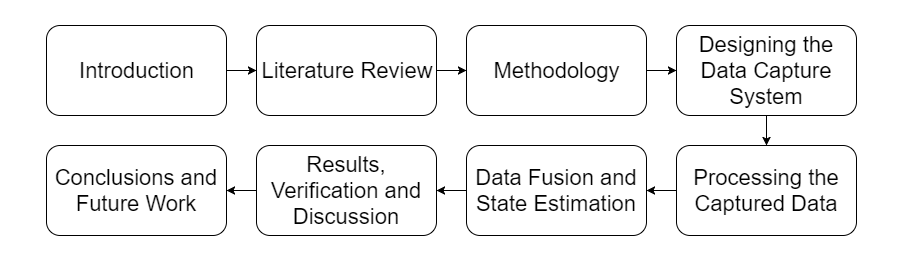
\includegraphics[width=\linewidth]{figures/introflow.png}
\caption{Flow chart outlining the report structure}
\label{fig:introflow}
\end{figure}